\chapter{Results}
\label{chapter:results}



\section{Performance Evaluation}

\begin{table}[htbp]
    \begin{footnotesize}
        \begin{tabularx}{\linewidth}{L|c|cc|ccc}
            \toprule
            \multirow{2}{*}{\textbf{Model}} & \multicolumn{6}{c}{\textbf{GQA}} \\
            \cmidrule{2-7}
            & Accuracy & Binary & Open & Validity & Plausibility & Distribution \\
            \midrule
            Human \cite{hudson2019gqa} & 89.30 & 91.20 & 87.40 & 98.90 & 97.20 & - \\
            \midrule
            LXMERT \cite{tan2019lxmert, tan2019lxmertgithub}& 59.80 & - & - & - & - & - \\
            BAN-4 \cite{kim2018bilinear, guo2019bilinear} & 61.95 & - & - & - & - & - \\
            GRN \cite{guo2019bilinear} & 64.22 & - & - & - & - & - \\
            MAC \cite{hudson2018compositional} & 73.64 & 81.86 & 65.94 & \textbf{95.38} & 92.46 & 2.05 \\
            \midrule
            \textbf{Our Model} & \textbf{90.30} & \textbf{91.59} & \textbf{89.10} & \textbf{95.35} & \textbf{94.48} & \textbf{0.29} \\
            \bottomrule
        \end{tabularx}
        \caption{A comparison of the performance of various models on the GQA validation set. Human performance is based on majority vote of 5 human responses for 4000 random GQA questions. For fair comparison, I report results for MAC using raw GloVe embeddings for each object, attribute and relation in the scene graph as its visual knowledge-base instead of object features. Where two citations are provided, the first corresponds to the original paper and the second corresponds to the source of the validation set results. }
    \end{footnotesize}
\end{table}

\section{Ablation Studies}
\label{sec:ablation_studies}

For all ablation studies in this chapter, I train models on the balanced GQA training set, I use the first half of the balanced validation set for parameter optimisation, and use the second half of the balanced validation set as a test set. All results reported in this section are computed on the second half of the balanced GQA validation set to avoid giving an unfair advantage to my best model, which was tuned using the first half of the balanced validation set.

\begin{figure}[htbp]
    \centering
    \begin{subfigure}[l]{0.5\textwidth}
        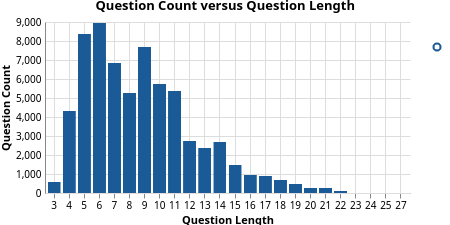
\includegraphics[width=\textwidth]{test_question_count_vs_question_length.png}
        \label{fig:test_question_length_distribution}
    \end{subfigure}
    \begin{subfigure}[r]{0.49\textwidth}
        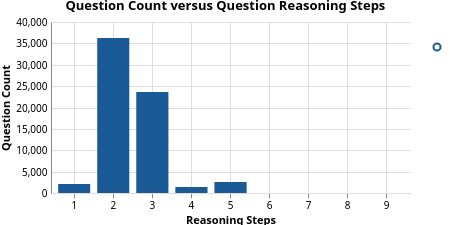
\includegraphics[width=\textwidth]{test_question_count_vs_reasoning_steps.png}
        \label{fig:test_reasoning_step_distribution}
    \end{subfigure}
    \caption{Distribution of questions across the second half of the balanced GQA validation set for both question length and reasoning step count.}
    \label{fig:test_reasoning_step_and_question_length_distribution}
\end{figure}



\subsection{Question Module Ablations}
\label{subsec:question_module_ablations}

\begin{table}[htbp]
\centering
\begin{footnotesize}
\begin{tabularx}{\linewidth}{CC|c|cc|ccc}
\toprule
\multirow{3}{0.1\textwidth}{\textbf{Question Module}} & \multirow{3}{0.1\textwidth}{\textbf{Scene Graph Module}} & \multicolumn{6}{c}{\multirow{2}{*}{\textbf{GQA}}}                                                                                                                                         \\
                                          &                                              & \multicolumn{6}{c}{}                                                                                                                                                                      \\ \cmidrule(l){3-8} 
                                          &                                              & \multicolumn{1}{l}{Accuracy} & \multicolumn{1}{l}{Binary} & \multicolumn{1}{l}{Open} & \multicolumn{1}{l}{Validity} & \multicolumn{1}{l}{Plausibility} & \multicolumn{1}{l}{Distribution} \\ \midrule
None                                      & GAT                                          & 86.52                        & 85.78                      & 87.21                    & 95.10                         & 93.85                            & 0.26                             \\
CNN                                       & GAT                                          & 87.35                        & 87.87                      & 86.86                    & 95.24                        & 94.22                            & 0.29                             \\
GAT                                       & GAT                                          & 89.43                        & \textbf{91.88}             & 87.16                    & 95.26                        & 94.19                            & 0.27                             \\
GCN                                       & GAT                                          & 86.02                        & 86.77                      & 85.32                    & 95.05                        & 93.92                            & 0.34                             \\
BiLSTM                                    & GAT                                          & \textbf{90.45}               & 91.73                      & \textbf{89.26}           & \textbf{95.34}                        & \textbf{94.48}                   & \textbf{0.19}                    \\
\bottomrule
\end{tabularx}
\end{footnotesize}
\end{table}



\begin{table}[htbp]
\centering
\begin{footnotesize}
\begin{tabular}{cc|c|ccccc}
\toprule
\multirow{3}{0.1\textwidth}{\textbf{Question Module}} & \multirow{3}{0.1\textwidth}{\textbf{Scene Graph Module}} & \multicolumn{6}{c}{\multirow{2}{*}{\textbf{GQA}}}                                                   \\
                                          &                                              & \multicolumn{6}{c}{}                                                                                \\ \cmidrule(l){3-8} 
                                          &                                              & Accuracy       & Query          & Compare        & Choose         & Logical        & Verify         \\ \midrule
None                                      & GAT                                          & 86.52          & 87.21          & 80.44          & 78.89          & 93.77          & 85.88          \\
CNN                                       & GAT                                          & 87.35          & 86.86          & 67.66          & 85.99          & 92.57          & 89.17          \\
GAT                                       & GAT                                          & 89.43          & 87.16          & \textbf{93.02} & 86.92          & 96.43          & 91.93          \\
GCN                                       & GAT                                          & 86.02          & 85.32          & 73.60          & 84.96          & 92.85          & 86.17          \\
BiLSTM                                    & GAT                                          & \textbf{90.45} & \textbf{89.26} & 69.69          & \textbf{90.87} & \textbf{97.45} & \textbf{92.10} \\ \bottomrule
\end{tabular}
\end{footnotesize}
\end{table}

{\color{red}Things to note: High compare score whenever we use the same question and scene graph module! e.g. GAT and GAT in this case}


\begin{table}[htbp]
\centering
\begin{footnotesize}
\begin{tabular}{cc|c|ccccc}
\toprule
\multirow{3}{0.1\textwidth}{\textbf{Question Module}} & \multirow{3}{0.1\textwidth}{\textbf{Scene Graph Module}} & \multicolumn{6}{c}{\multirow{2}{*}{\textbf{GQA}}}                                                   \\
                                          &                                              & \multicolumn{6}{c}{}                                                                                \\ \cmidrule(l){3-8} 
                                          &                                              & Accuracy       & Global         & Object         & Attribute      & Relation       & Category       \\ \midrule
None                                      & GAT                                          & 86.52          & \textbf{83.97}          & 94.75          & 87.35          & 83.67          & 89.01          \\
CNN                                       & GAT                                          & 87.35          & 83.78          & 93.63          & 85.37          & 87.37          & 87.14          \\
GAT                                       & GAT                                          & 89.43          & 83.82          & 97.24          & \textbf{89.74} & 87.88          & 87.62          \\
GCN                                       & GAT                                          & 86.02          & 83.39          & 93.36          & 83.65          & 86.32          & 83.43          \\
BiLSTM                                    & GAT                                          & \textbf{90.45} & 83.92          & \textbf{97.39} & 88.39          & \textbf{90.51} & \textbf{90.65} \\ \bottomrule
\end{tabular}
\end{footnotesize}
\end{table}

\begin{figure}[htbp]
    \centering
    \begin{subfigure}[l]{0.5\textwidth}
        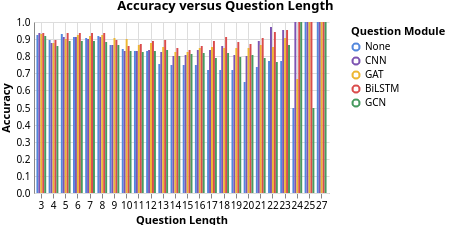
\includegraphics[width=\textwidth]{test_accuracy_vs_question_length_question_ablation.png}
        \label{fig:test_accuracy_vs_question_length_question_ablation}
    \end{subfigure}
    \begin{subfigure}[r]{0.49\textwidth}
        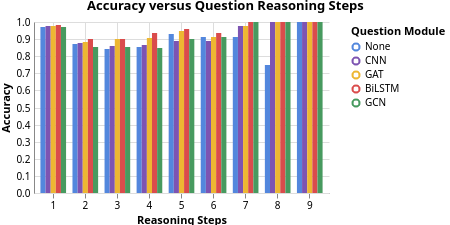
\includegraphics[width=\textwidth]{test_accuracy_vs_reasoning_steps_question_ablation.png}
        \label{fig:test_accuracy_vs_reasoning_steps_question_ablation}
    \end{subfigure}
    \caption{Per-question-length and per-reasoning-step accuracy for various question processing module types.}
\end{figure}

The high performance of the right-hand tails in both cases are due to the small number of questions with a large number of words or reasoning steps, as illustrated in \figureautorefname{ \ref{fig:test_reasoning_step_and_question_length_distribution}}

\subsection{Scene Graph Module Ablations}
\label{subsec:scene_graph_module_ablations}

\begin{table}[htbp]
\centering
\begin{footnotesize}
\begin{tabularx}{\linewidth}{CC|c|cc|ccc}
\toprule
\multirow{3}{0.1\textwidth}{\textbf{Question Module}} & \multirow{3}{0.1\textwidth}{\textbf{Scene Graph Module}} & \multicolumn{6}{c}{\multirow{2}{*}{\textbf{GQA}}}                                                                                                                                         \\
                                          &                                              & \multicolumn{6}{c}{}                                                                                                                                                                      \\ \cmidrule(l){3-8} 
                                          &                                              & \multicolumn{1}{l}{Accuracy} & \multicolumn{1}{l}{Binary} & \multicolumn{1}{l}{Open} & \multicolumn{1}{l}{Validity} & \multicolumn{1}{l}{Plausibility} & \multicolumn{1}{l}{Distribution} \\ \midrule
BiLSTM                                    & None                                         & 73.63                        & 81.84                      & 65.98                    & \textbf{95.38}               & 92.46                            & 1.09                    \\
BiLSTM                                    & BiLSTM                                       & 83.35                        & 85.81                      & 81.06                    & 95.27                        & 93.73                            & 0.31                             \\
BiLSTM                                    & GCN                                          & 69.44                        & 78.14                      & 61.34                    & 95.13                        & 91.95                            & 1.11                             \\
BiLSTM                                    & GAT                                          & \textbf{90.45}               & \textbf{91.73}                      & \textbf{89.26}           & 95.34                        & \textbf{94.48}                   & \textbf{0.19}                    \\
\bottomrule
\end{tabularx}
\end{footnotesize}
\end{table}

\begin{table}[htbp]
\centering
\begin{footnotesize}
\begin{tabular}{cc|c|ccccc}
\toprule
\multirow{3}{0.1\textwidth}{\textbf{Question Module}} & \multirow{3}{0.1\textwidth}{\textbf{Scene Graph Module}} & \multicolumn{6}{c}{\multirow{2}{*}{\textbf{GQA}}}                                                   \\
                                          &                                              & \multicolumn{6}{c}{}                                                                                \\ \cmidrule(l){3-8} 
                                          &                                              & Accuracy       & Query          & Compare        & Choose         & Logical        & Verify         \\ \midrule
BiLSTM                                    & None                                         & 73.63          & 65.98          & 69.44          & 72.84          & 92.85          & 82.44          \\
BiLSTM                                    & BiLSTM                                       & 83.35          & 81.06          & \textbf{92.22}          & 73.98          & 95.79          & 85.91          \\
BiLSTM                                    & GCN                                          & 69.44          & 61.34          & 66.37          & 71.04          & 85.96          & 79.43          \\
BiLSTM                                    & GAT                                          & \textbf{90.45} & \textbf{89.26} & 69.69          & \textbf{90.87} & \textbf{97.45} & \textbf{92.10} \\ \bottomrule
\end{tabular}
\end{footnotesize}
\end{table}

\begin{table}[htbp]
\centering
\begin{footnotesize}
\begin{tabular}{cc|c|ccccc}
\toprule
\multirow{3}{0.1\textwidth}{\textbf{Question Module}} & \multirow{3}{0.1\textwidth}{\textbf{Scene Graph Module}} & \multicolumn{6}{c}{\multirow{2}{*}{\textbf{GQA}}}                                                   \\
                                          &                                              & \multicolumn{6}{c}{}                                                                                \\ \cmidrule(l){3-8} 
                                          &                                              & Accuracy       & Global         & Object         & Attribute      & Relation       & Category       \\ \midrule
BiLSTM                                    & None                                         & 73.63          & \textbf{85.18} & 95.15          & 64.46          & 72.38          & 82.54          \\
BiLSTM                                    & BiLSTM                                       & 83.35          & 82.86          & 95.60          & 80.88          & 81.02          & 89.92          \\
BiLSTM                                    & GAT                                          & \textbf{90.45} & 83.92          & \textbf{97.39} & \textbf{88.39}          & \textbf{90.51} & \textbf{90.65} \\
BiLSTM                                    & GCN                                          & 69.44          & 70.45          & 87.54          & 67.22          & 66.25          & 69.77          \\
\bottomrule
\end{tabular}
\end{footnotesize}
\end{table}


\begin{figure}[htbp]
    \centering
    \begin{subfigure}[l]{0.5\textwidth}
        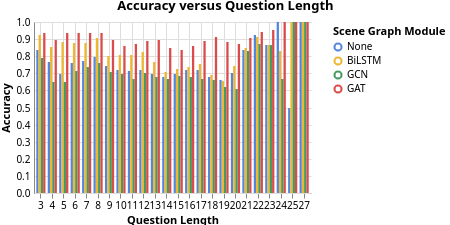
\includegraphics[width=\textwidth]{test_accuracy_vs_question_length_scene_ablation.png}
        \label{fig:test_accuracy_vs_question_length_scene_ablation}
    \end{subfigure}
    \begin{subfigure}[r]{0.49\textwidth}
        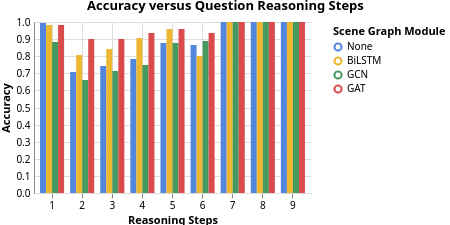
\includegraphics[width=\textwidth]{test_accuracy_vs_reasoning_length_scene_ablation.png}
        \label{fig:test_accuracy_vs_reasoning_steps_scene_ablation}
    \end{subfigure}
    \caption{Per-question-length and per-reasoning-step accuracy for various scene graph processing module types.}
\end{figure}

The high performance of the right-hand tails in both cases are due to the small number of questions with a large number of words or reasoning steps, as illustrated in \figureautorefname{ \ref{fig:test_reasoning_step_and_question_length_distribution}}


{\color{red}Things to note: High compare score whenever we use the same question and scene graph module! e.g. BiLSTM and BiLSTM in this case}

{\color{red}TODO: GloVe only for scene graph and questions}

{\color{red}TODO: Ablations on scene graph embedding for best model only:
\begin{itemize}
    \item Removal of skip-edges in the graph
    \item Removal of relation data, with edges only occurring between objects where a relation would usually be (i.e. skip edges w/ no relation nodes)
    \item If time, removal of relation and attribute data as well.
\end{itemize}}

\begin{itemize}
    \item Includes more important initial tests, move less important ones to appendix.
\end{itemize}

\begin{itemize}
    \item GloVe vs random normal distribution. Glove required less tuning since the vector norms already worked well.
\end{itemize}

\section{Hyperparameter Optimisation}
\label{sec:hyperparameter_optimisation}

These results represent a total of 55 days of GPU compute

{\color{red}
  \begin{itemize}
    \item \textit{Weights \& Biases} \cite{wandb} implementation of bayesian optimisation, using the hyperband early stopping method
    \item Include results using LeakyReLU between GAT layers?
  \end{itemize}
}



The effects of the Hyperband method are clearly seen in \figureautorefname{ \ref{fig:hyperparameter_optimisation_validation_loss_and_accuracy}}, where only a few models are trained to completion and less promising models are stopped earlier to encourage exploration of the hyperparameter search space.

\begin{figure}
    \centering
    \begin{subfigure}[t]{\textwidth}
        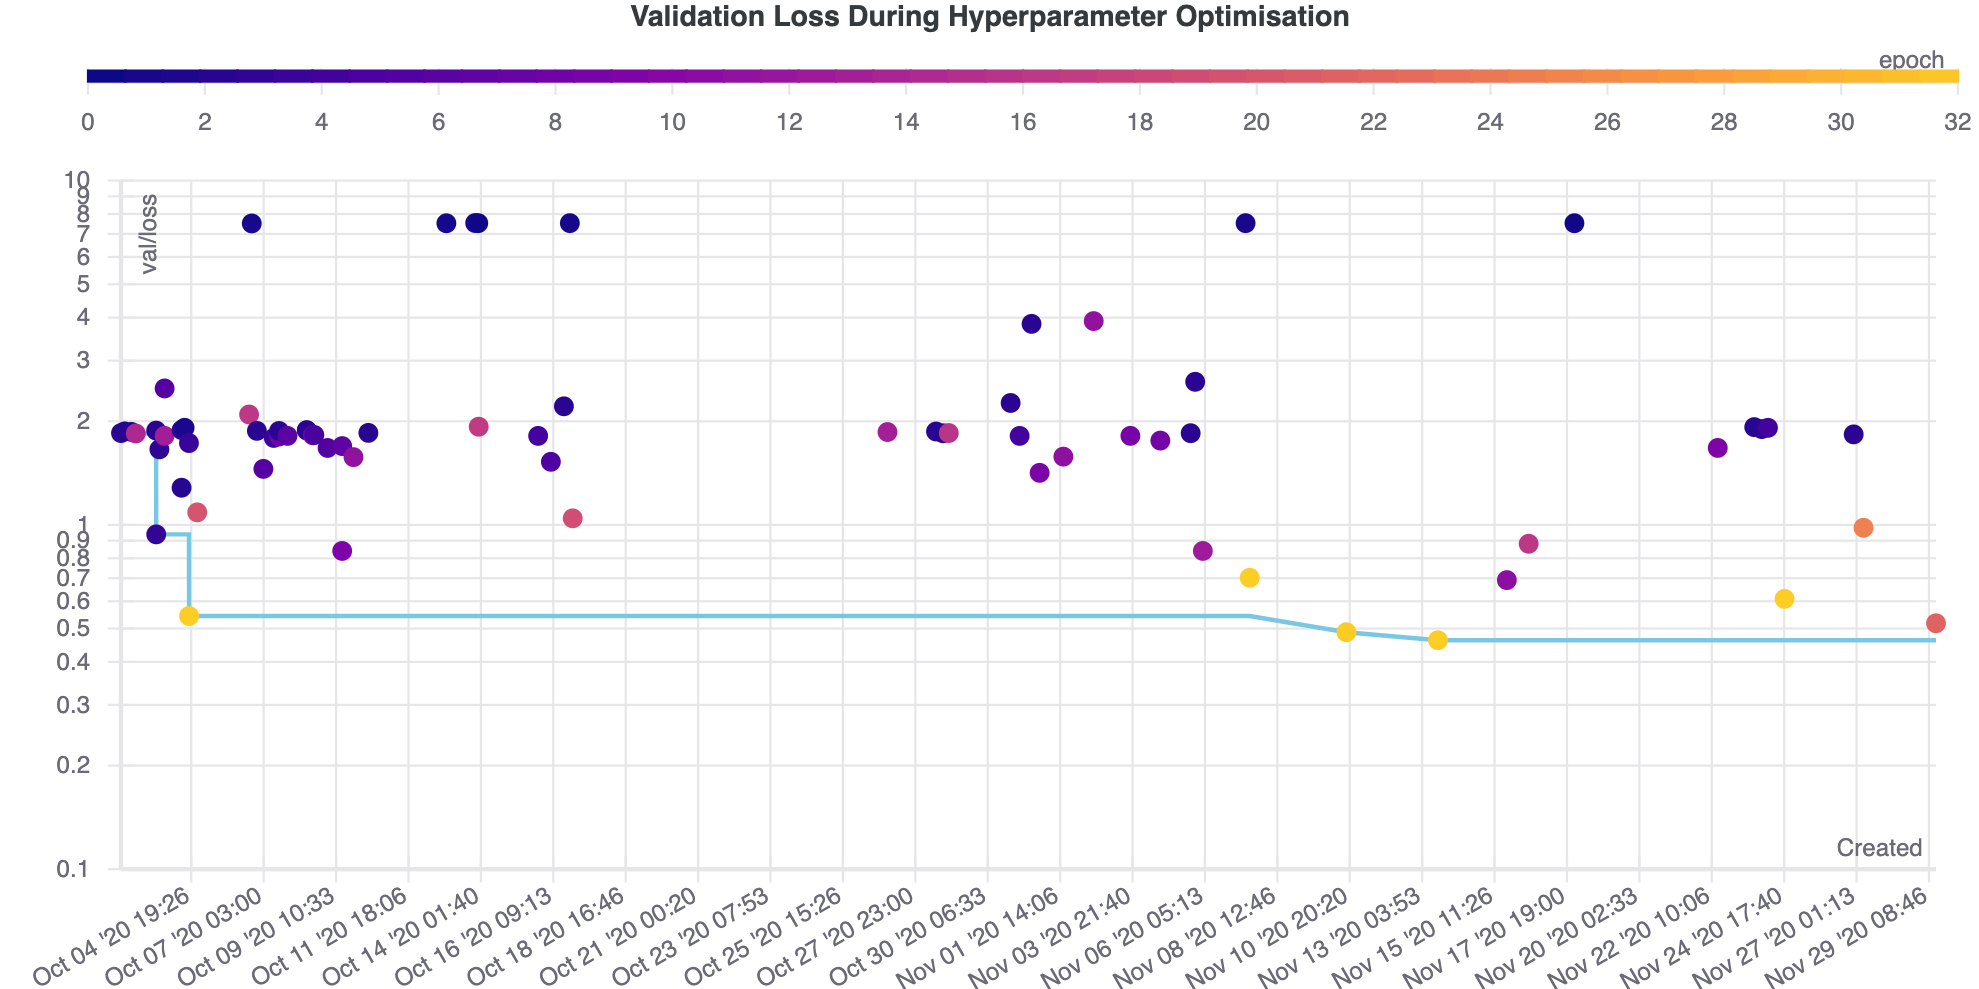
\includegraphics[width=\textwidth]{hyperparameter_optimisation_validation_loss.png}
        \label{fig:hyperparameter_optimisation_validation_loss}
        \caption{Validation loss throughout the hyperparameter optimisation process.}
    \end{subfigure}
    \par\bigskip % force a bit of vertical whitespace
    \par\bigskip
    \begin{subfigure}[b]{\textwidth}
        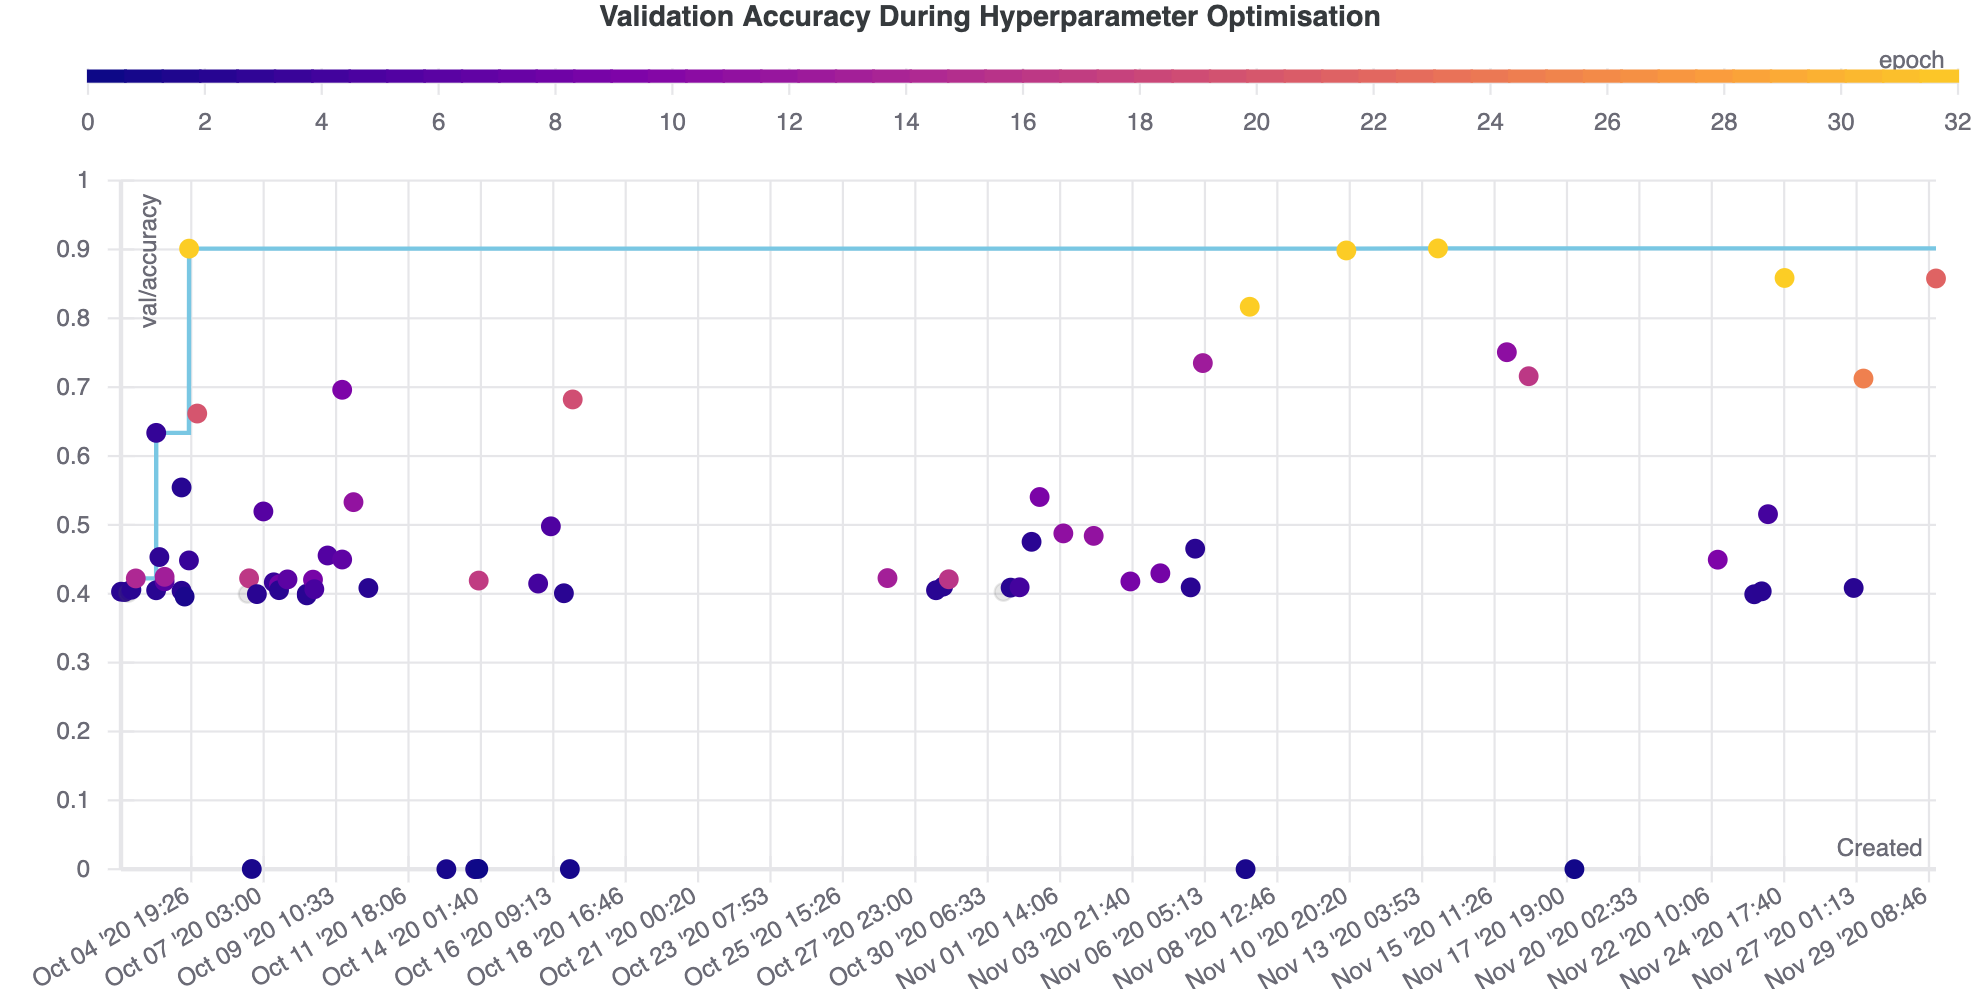
\includegraphics[width=\textwidth]{hyperparameter_optimisation_validation_accuracy.png}
        \label{fig:hyperparameter_optimisation_validation_accuracy}
        \caption{Validation accuracy throughout the hyperparameter optimisation process. Greyed out points correspond to models with a loss greater than 10.}
    \end{subfigure}
    \caption{A summary of validation loss and accuracy throughout the hyperparameter optimisation process. Each point represents a trained model, and its colour indicates how many epochs the model was trained for.}
    \label{fig:hyperparameter_optimisation_validation_loss_and_accuracy}
\end{figure}

\begin{figure}
    \centering
    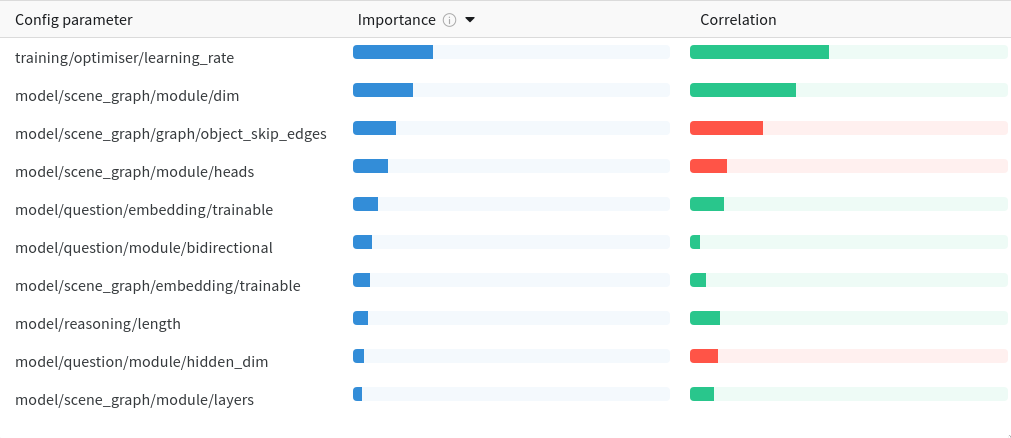
\includegraphics[width=\textwidth]{hyperparam_importance_and_correlation.png}
    \caption{Hyperparameter importance with respect to validation loss. Correlation is the linear correlation between each parameter and the validation loss, between -1 and 1. Parameter importance a value between 0 and 1, estimated by \textit{Weights \& Biases} \cite{wandb} by training a random forest classifier using configuration parameters as features and the validation loss as the target prediction.}
    \label{fig:hyperparam_importance_and_correlation}
\end{figure}

{\color{red} TODO: Correlation does not necessarily imply causation for parameter correlation to validation loss in \figureautorefname{ \ref{fig:hyperparam_importance_and_correlation}}}

\begin{figure}
    \centering
    \begin{subfigure}[l]{0.5\textwidth}
        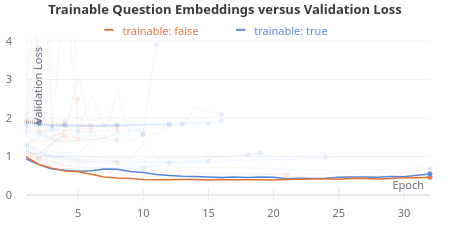
\includegraphics[width=\textwidth]{hyperparam_trainable_question_embedding_loss.png}
        \label{fig:hyperparam_trainable_question_embedding_loss}
        \caption{Validation Loss}
    \end{subfigure}
    \begin{subfigure}[r]{0.49\textwidth}
        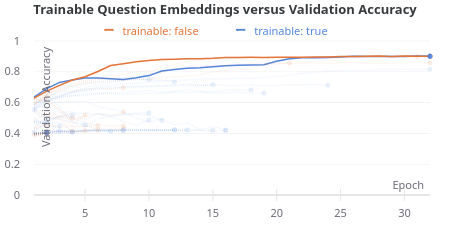
\includegraphics[width=\textwidth]{hyperparam_trainable_question_embedding_accuracy.png}
        \label{fig:hyperparam_trainable_question_embedding_accuracy}
        \caption{Validation Accuracy}
    \end{subfigure}
    \caption{}
    \label{fig:hyperparam_trainable_question_embedding_loss_and_accuracy}
\end{figure}
 
\begin{figure}
    \centering
    \begin{subfigure}[l]{0.5\textwidth}
        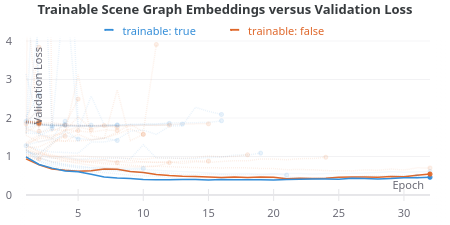
\includegraphics[width=\textwidth]{hyperparam_trainable_scene_embedding_loss.png}
        \label{fig:hyperparam_trainable_scene_embedding_loss}
        \caption{Validation Loss}
    \end{subfigure}
    \begin{subfigure}[r]{0.49\textwidth}
        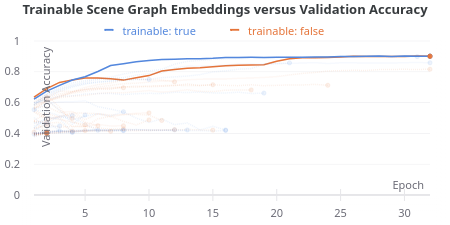
\includegraphics[width=\textwidth]{hyperparam_trainable_scene_embedding_accuracy.png}
        \label{fig:hyperparam_trainable_scene_embedding_accuracy}
        \caption{Validation Accuracy}
    \end{subfigure}
    \caption{}
    \label{fig:hyperparam_trainable_scene_embedding_loss_and_accuracy}
\end{figure}

\begin{figure}
    \centering
    \begin{subfigure}[l]{0.5\textwidth}
        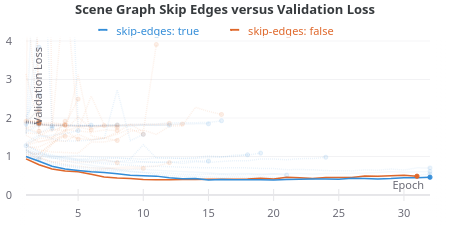
\includegraphics[width=\textwidth]{hyperparam_skip_edges_loss.png}
        \label{fig:hyperparam_skip_edges_loss}
        \caption{Validation Loss}
    \end{subfigure}
    \begin{subfigure}[r]{0.49\textwidth}
        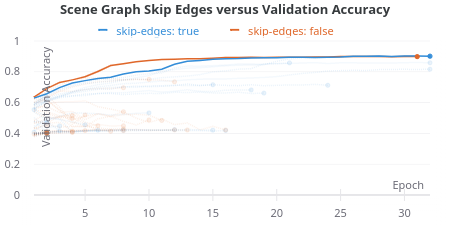
\includegraphics[width=\textwidth]{hyperparam_skip_edges_accuracy.png}
        \label{fig:hyperparam_skip_edges_accuracy}
        \caption{Validation Accuracy}
    \end{subfigure}
    \caption{}
    \label{fig:hyperparam_skip_edges_loss_and_accuracy}
\end{figure}
